\documentclass[dvipdfmx,a4paper]{jsarticle}
\usepackage{amsmath,amssymb}
\usepackage{amsthm}
\usepackage{bm}
\usepackage[dvipdfmx]{graphicx}
\usepackage{ascmac}
\usepackage{subfigure}
\usepackage{verbatim}
\usepackage{wrapfig}
\usepackage{makeidx}
\usepackage[dvipdfmx]{hyperref}
\usepackage{setspace}
\usepackage{color}
\usepackage{listings}
\usepackage{cleveref}
\usepackage{mathtools}
\usepackage{framed}
\usepackage[textwidth=50zw,lines=46]{geometry}
\usepackage{here}

\usepackage{listings, jlisting, color}
\definecolor{OliveGreen}{rgb}{0.0,0.6,0.0}
\definecolor{Orenge}{rgb}{0.89,0.55,0}
\definecolor{SkyBlue}{rgb}{0.28, 0.28, 0.95}
\lstset{
  language={C++}, % 言語の指定
  basicstyle={\ttfamily},
  identifierstyle={\small},
  commentstyle={\smallitshape},
  keywordstyle={\small\bfseries},
  ndkeywordstyle={\small},
  stringstyle={\small\ttfamily},
  frame={tb},
  breaklines=true,
  columns=[l]{fullflexible},
  numbers=left,
  xrightmargin=0zw,
  xleftmargin=3zw,
  numberstyle={\scriptsize},
  stepnumber=1,
  numbersep=1zw,
  lineskip=-0.5ex,
  keywordstyle={\color{SkyBlue}},     %キーワード(int, ifなど)の書体指定
  commentstyle={\color{OliveGreen}},  %注釈の書体
  stringstyle=\color{Orenge}          %文字列
}

\begin{document}

\title{課題演習C3\quad レポート (1回目) }
\author{0500-34-0042\quad 大平 達也}
\date{\today}
\maketitle

\section{目的}
系外惑星TOI1516 bのTransit検出を目標とする。分かっている, 観測日におけるターゲットの情報は以下の通り: 
\begin{description}
  \item[観測日] 2024/11/11
  \item[ingress] 20:00
  \item[degrees] 22:50
  \item[視等級] 10.8 mag
  \item[減光量] 0.016 mag
\end{description}
今回は, ingressの途中から観測を始めた。
\section{これまでの進捗状況}
\subsection{データの一次処理}
IRAFを用いて, 11/11に取得した観測データの一次処理を行った。
\subsection{測光用コードの開発}
途中までIRAFのスクリプトを書いていたが, 途中からPythonでの開発に切り替えた。作成したコードは以下の通り。なおアパーチャーの半径はHWHMの1.2倍とした。 

\begin{lstlisting}[caption=開口測光用のコード, label=apphot, language=Python]
import glob
from astropy.io import fits
from astropy.time import Time
from photutils.aperture import CircularAperture, CircularAnnulus, aperture_photometry
from photutils.detection import DAOStarFinder
from astropy.stats import mad_std
import numpy as np
import matplotlib.pyplot as plt
from zoneinfo import ZoneInfo
from datetime import timezone
import pandas as pd
import matplotlib.dates as mdates

# 重心座標を検出するための関数を定義
def find_star_position(data, initial_pos, search_radius, fwhm=3.0, threshold=5.0):
    """
    初期位置近辺で星を検出し、正確な座標と検出された星の情報を返す関数
    """
    # 背景ノイズの推定
    bkg_sigma = mad_std(data)
    
    # 星の検出
    daofind = DAOStarFinder(fwhm=fwhm, threshold=threshold * bkg_sigma)
    sources = daofind(data - np.median(data))
    
    if sources is None or len(sources) == 0:
        print(f"No sources found around position {initial_pos}")
        return initial_pos, None  # 検出できなかった場合は初期位置とNoneを返す
    
    # 初期位置からの距離を計算
    distances = np.sqrt((sources['xcentroid'] - initial_pos[0])**2 + 
                        (sources['ycentroid'] - initial_pos[1])**2)
    
    # 検出範囲内の星をフィルタ
    within_radius = distances < search_radius
    if not np.any(within_radius):
        print(f"No sources within {search_radius}px of position {initial_pos}")
        return initial_pos, None  # 見つからない場合は初期位置とNoneを返す
    
    # 検出された星の中で最も明るいものを選択
    brightest = sources[within_radius][sources['flux'][within_radius].argmax()]
    
    return (brightest['xcentroid'], brightest['ycentroid']), brightest
    
# 検索範囲 (pxl) 
search_radius = 15

# 結果を保存するリスト
times = []
rel_mags = []
errors = []
target_mags = []

# ターゲット星, 参照星の座標の初期値を入力
target_initial = (376.00, 295.00)
comp_initials = [
    (477.00, 324.00), 
    (474.00, 250.00), 
    (310.00, 190.00), 
    (227.00, 371.00)
]

# 参照星の数を取得
num_comps = len(comp_initials)

# 各参照星のフラックスを保存するリストのリストを作成
comp_fluxes_list = [[] for _ in range(num_comps)]


# FITSファイルのリストを取得(日時順にソート)
fits_files = sorted(glob.glob('./data/10toi1516a010*.fit'))

# ターゲット星と参照星の現在の位置
target_position = target_initial
comp_positions = comp_initials.copy()

# 各画像での処理
for idx, file in enumerate(fits_files):
    print(f"Processing {file} ({idx+1}/{len(fits_files)})")
    try:
        with fits.open(file) as hdu:
            data = hdu[0].data
            header = hdu[0].header
    except Exception as e:
        print(f"Error opening {file}: {e}")
        for flux_list in comp_fluxes_list:
            flux_list.append(np.nan)
        target_mags.append(np.nan)
        continue
    
    # 観測時刻を取得
    if 'DATE-OBS' in header:
        time_utc = Time(header['DATE-OBS']).to_datetime(timezone=timezone.utc)
        time_jst = time_utc.astimezone(ZoneInfo('Asia/Tokyo'))
    else:
        print(f"DATE-OBS not found in {file}. Skipping.")
        for flux_list in comp_fluxes_list:
            flux_list.append(np.nan)
        target_mags.append(np.nan)
        continue
    times.append(time_jst)
    
    # ターゲット星の位置と明るい星の情報を取得
    target_position, brightest_star = find_star_position(data, target_position, search_radius=search_radius)
    
    # FWHMの取得
    if brightest_star is not None and 'fwhm' in brightest_star:
        measured_fwhm = brightest_star['fwhm']
        aperture_radius = measured_fwhm * 1.5  # FWHMの1.5倍をアパーチャ半径とする
    else:
        aperture_radius = 6  # デフォルト値
    
    # 参照星の位置を検索
    for i, comp_pos in enumerate(comp_positions):
        comp_positions[i], _ = find_star_position(data, comp_pos, search_radius=search_radius)
    
    # 測光アパーチャーを定義(動的に設定した半径を使用)
    positions = [target_position] + comp_positions
    apertures = CircularAperture(positions, r=aperture_radius)
    
    # アパーチャで測光を実行
    phot_table_apertures = aperture_photometry(data, apertures)
    
    # 背景補正用アノラスを定義(各アパーチャに対して1つのアノラスを作成)
    annuli = CircularAnnulus(positions, r_in=aperture_radius + 1, r_out=aperture_radius + 4)
    
    # アノラスで測光を実行
    phot_table_annuli = aperture_photometry(data, annuli)
    
    # 各アパーチャに対応するアノラスのフラックスを取得
    # annuli.areaは全アノラスの面積のリストを返す
    bkg_fluxes = phot_table_annuli['aperture_sum'] / annuli.area * apertures.area
    
    # アパーチャ内の背景を差し引いたフラックスを計算
    target_flux = phot_table_apertures['aperture_sum'][0] - bkg_fluxes[0]
    comp_fluxes = phot_table_apertures['aperture_sum'][1:] - bkg_fluxes[1:]
    
    # フラックスが負になる場合は np.nan に設定
    target_flux = target_flux if target_flux > 0 else np.nan
    comp_fluxes = np.where(comp_fluxes > 0, comp_fluxes, np.nan)
    
    # 相対等級を計算
    if not np.isnan(target_flux) and not np.isnan(comp_fluxes).all():
        comp_flux = np.nanmean(comp_fluxes)
        if comp_flux > 0:
            rel_mag = -2.5 * np.log10(target_flux / comp_flux)
        else:
            rel_mag = np.nan
    else:
        rel_mag = np.nan
    rel_mags.append(rel_mag)

    # 機械等級を計算
    if not np.isnan(target_flux) and target_flux > 0:
        target_mag = -2.5 * np.log10(target_flux)
    else:
        target_mag = np.nan
    target_mags.append(target_mag)
    
    # 誤差の推定
    if not np.isnan(comp_flux):
        error = np.nanstd(comp_fluxes / comp_flux)
    else:
        error = np.nan
    errors.append(error)
    
    # 各参照星のフラックスをリストに追加
    for i, flux in enumerate(comp_fluxes):
        comp_fluxes_list[i].append(flux)
        print(f'Comparison Star {i+1}: Flux = {flux}')
\end{lstlisting}

\subsection{測光結果}
相対測光により, TOI1516の等級を各画像で求めた。これをplotしたものを図\ref{fig:toi1516}に示す。

\begin{figure}[H]
  \centering
  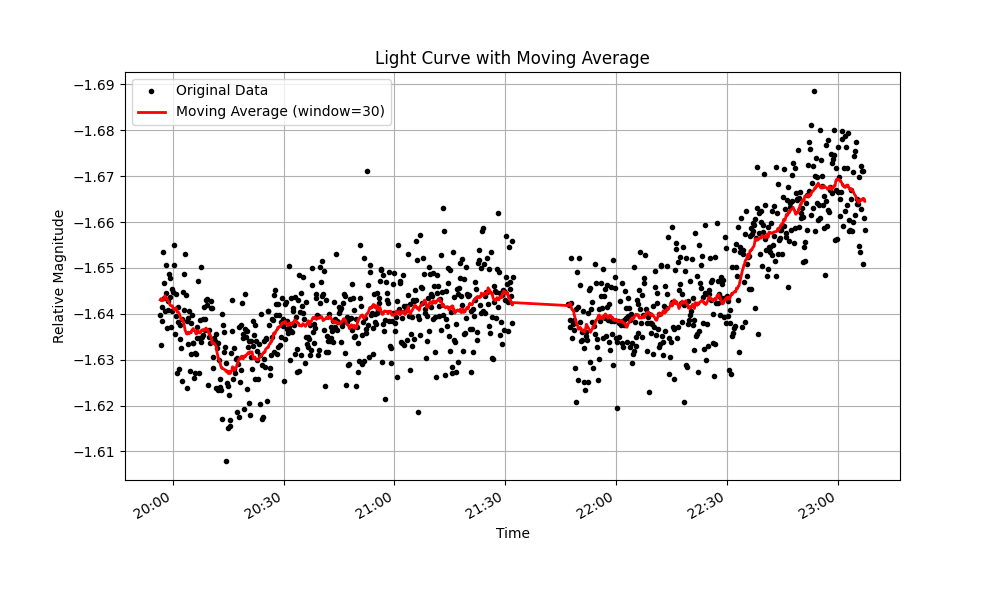
\includegraphics[width=0.9\textwidth]{./fig/light_curve_toi1516_with_moving_average.png}
  \caption{TOI1516の光度曲線}
  \label{fig:toi1516}
\end{figure}

\subsection{参照星の選び方について}
参照星は, 常に視野内に位置し, ターゲット星と同程度の明るさのものを選んだ。また, 測光したのちに, 参照星の等級の時間変化を調べ, 参照星として適切であるか検証した。

たとえば, 最初に選んだ参照星の等級の時間変化は図\ref{fig:comp}であった。全体として同じようなトレンドではあるが, Comp 4 (紫) のみノイズが大きいように見える。実際, Comp 4が参照星の中で最も暗い星であったことから, 参照星として選ぶのは適切でないと判断し, 他の参照星を選んだ。これを繰り返すことで, 最終的な参照星を選んだ。

なお, 参考までに, TOI1516の高度からエアマスを計算したplotも掲載しておく (図\ref{fig:airmass})。観測データから, 参照星の等級は時間とともに暗い方へ変化していったためエアマスには反する結果となった。原因は不明。

\begin{figure}[H]
  \centering
  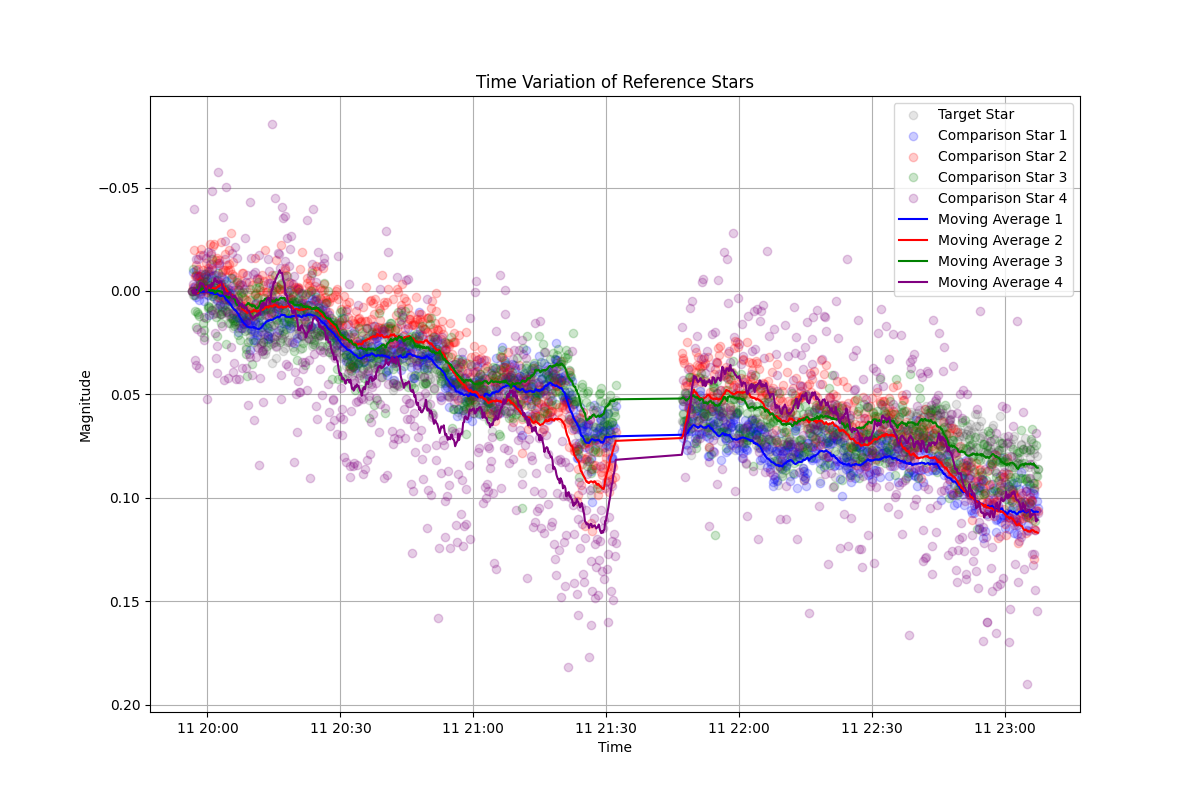
\includegraphics[width=0.9\textwidth]{./fig/light_curve_comp_first.png}
  \caption{参照星の光度曲線}
  \label{fig:comp}
\end{figure}

\begin{figure}[H]
  \centering
  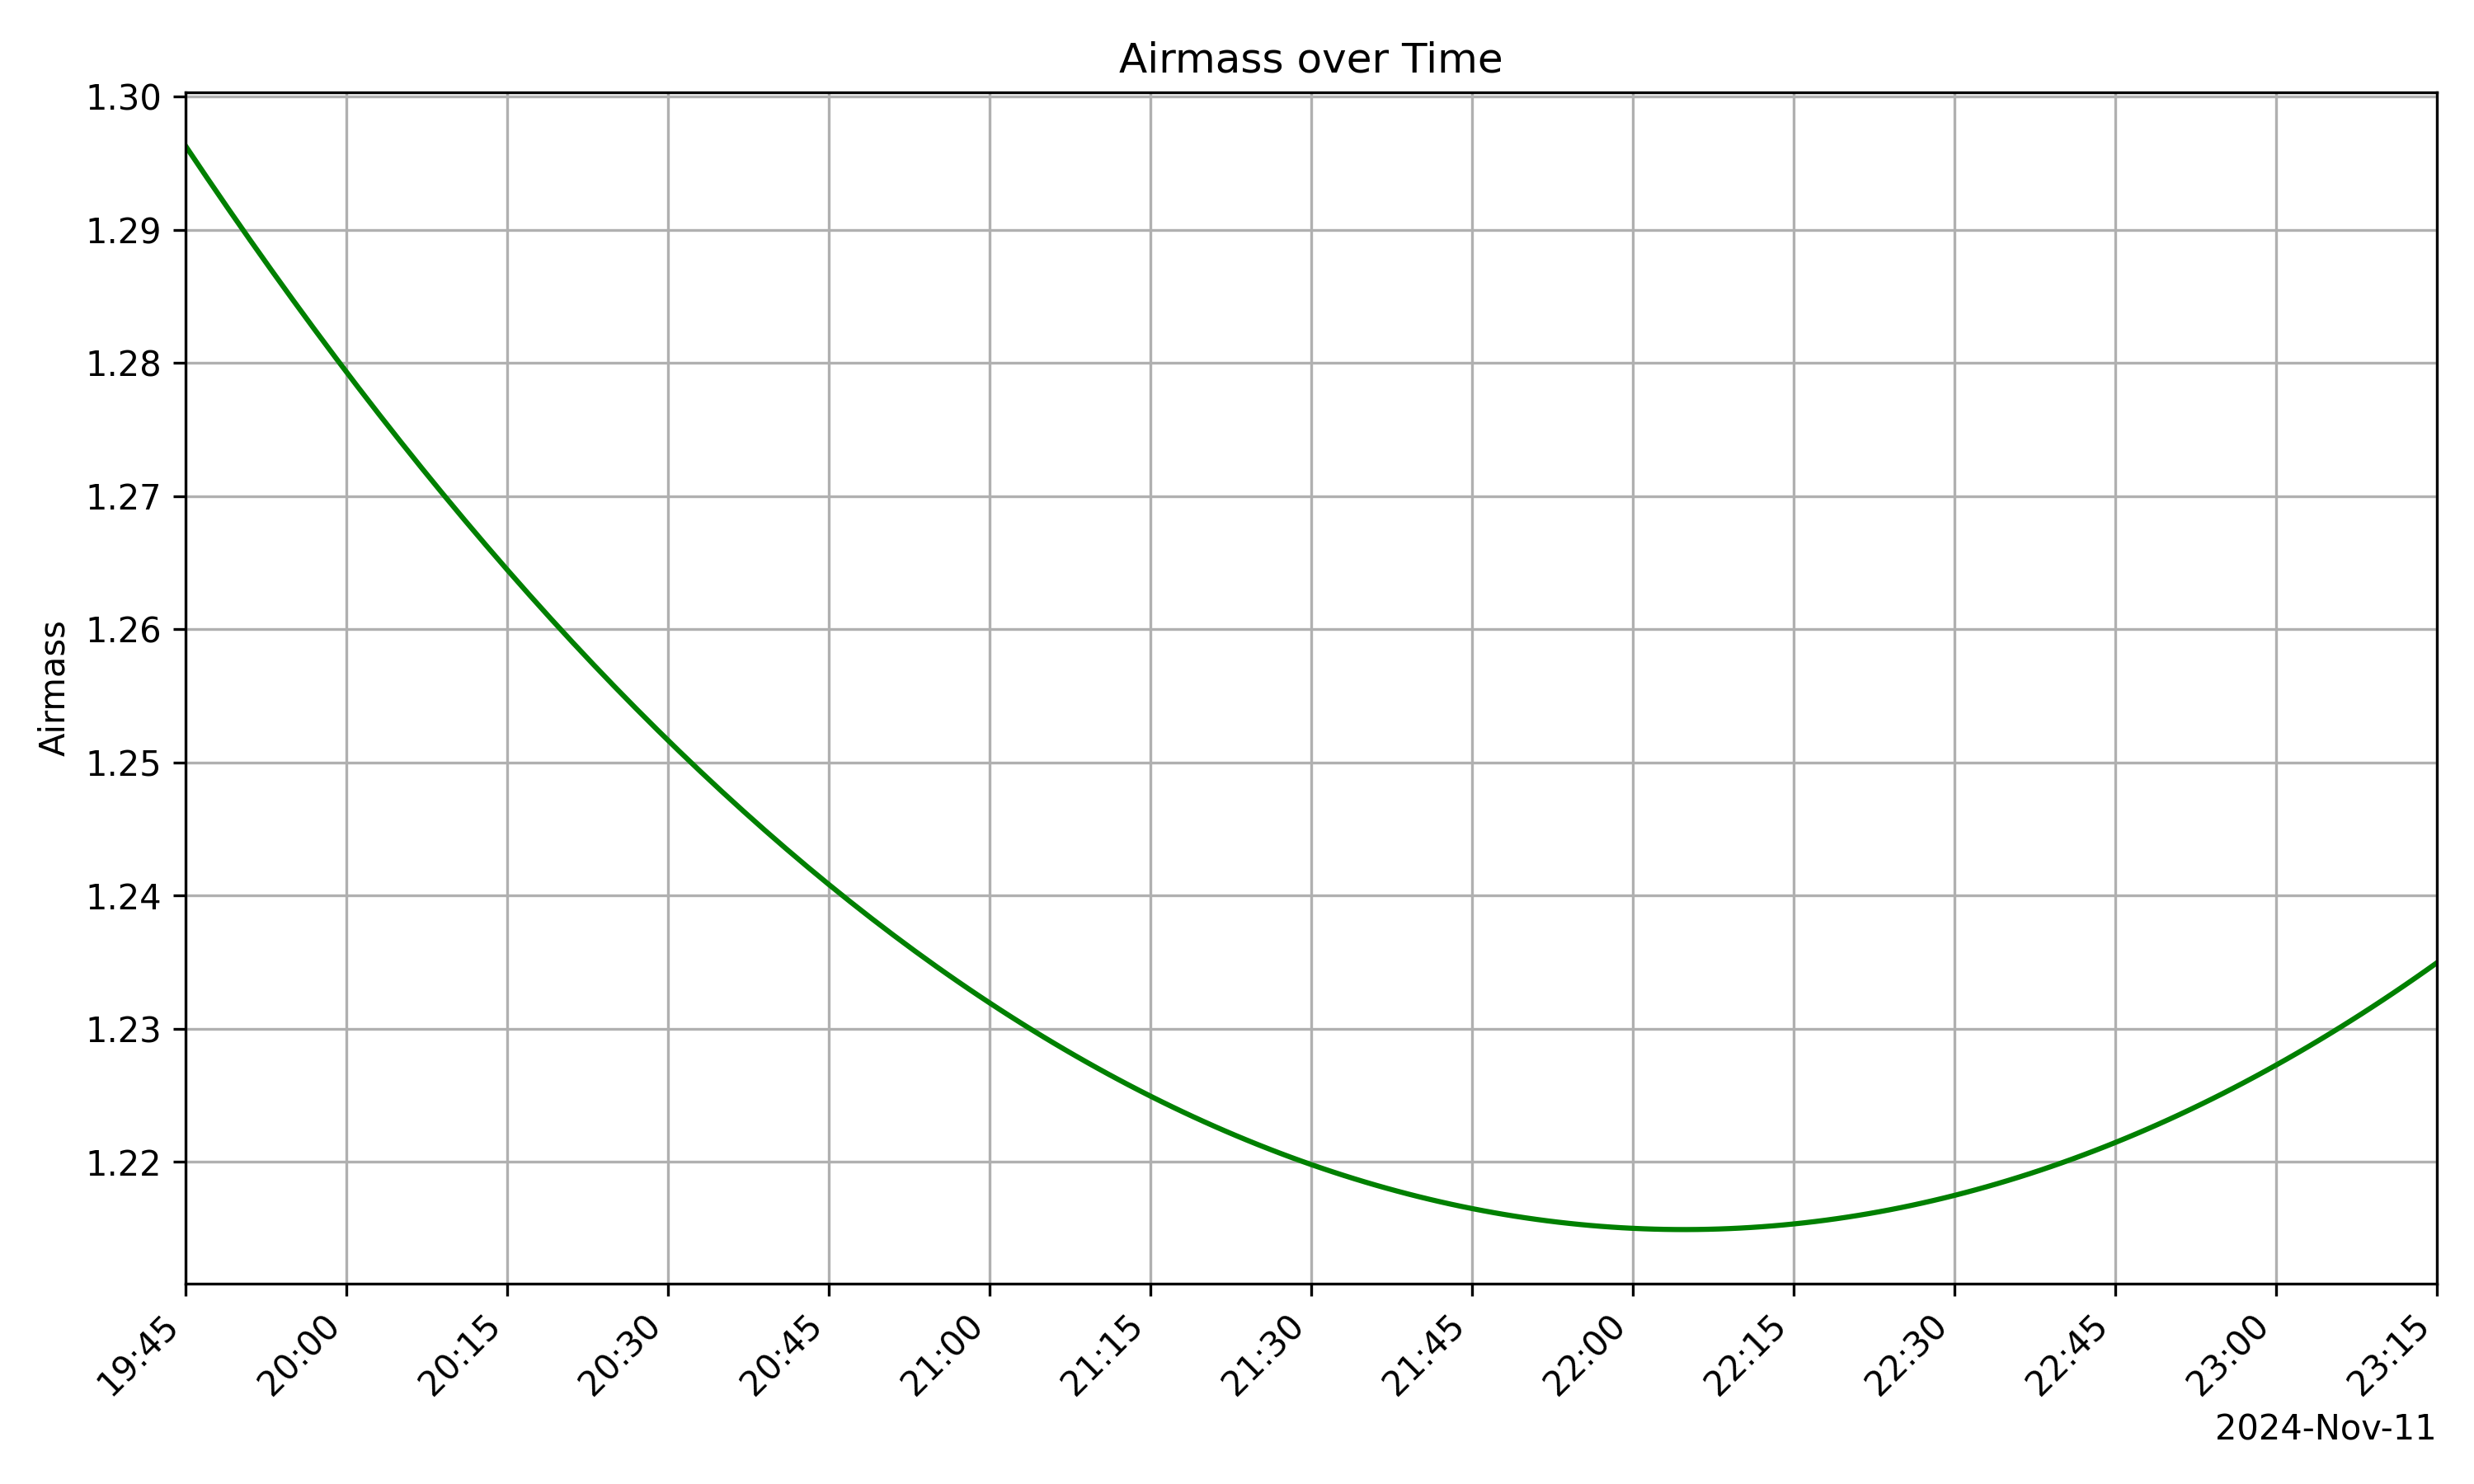
\includegraphics[width=0.9\textwidth]{./fig/airmass_over_time.png}
  \caption{エアマスの時間変化}
  \label{fig:airmass}
\end{figure}

\section{今後の予定}
PSF測光とかしてみたいです。
\end{document}